% --- SAM 1, SAM 2, and SAM 3 ---
\begin{frame}{Segment Anything Model (SAM): Promptable Segmentation}
  \centering
  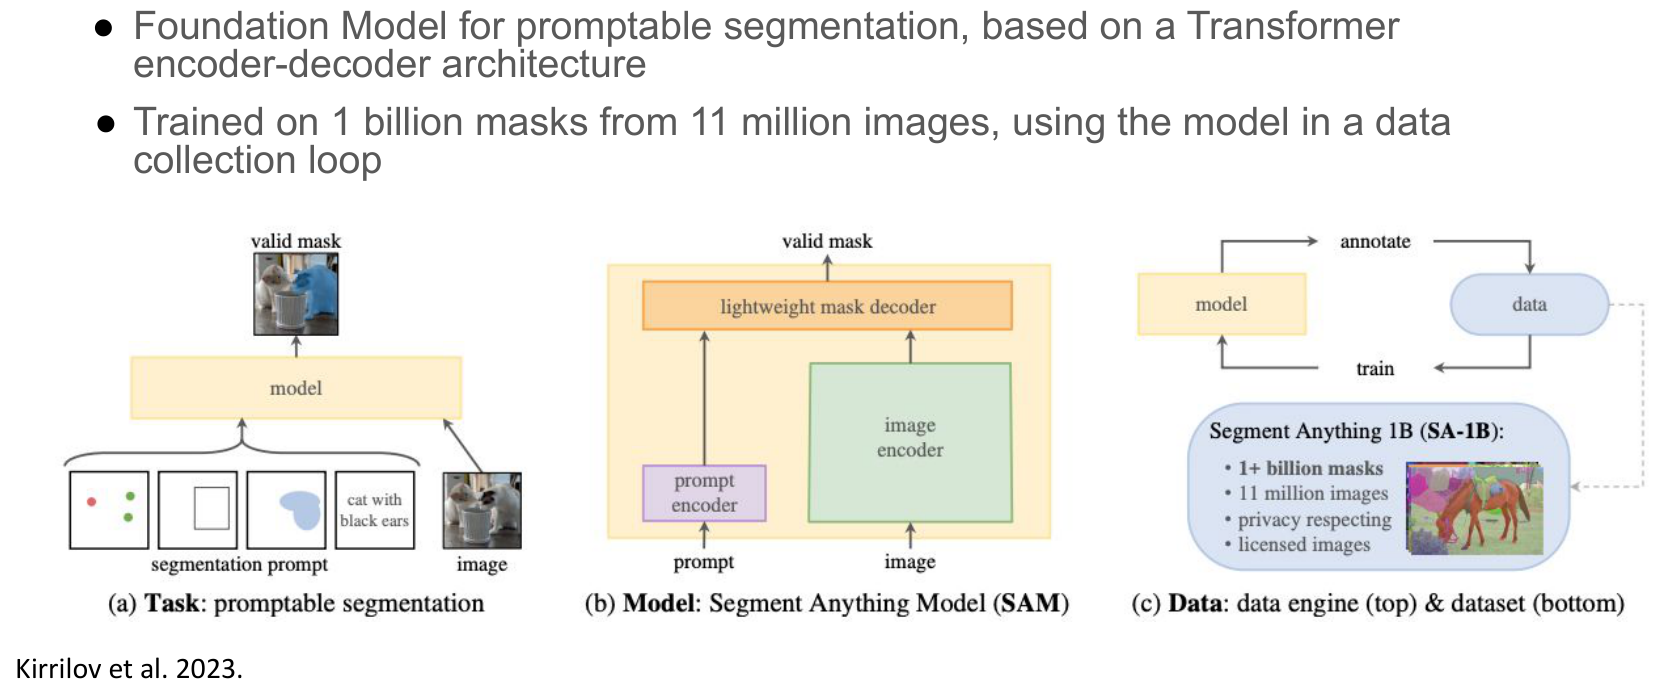
\includegraphics[width=\textwidth,height=0.80\textheight,keepaspectratio]{images/foundation-models/sam_promptable_segmentation_overview.png}\\[0.1em]
  {\scriptsize Stanford BIODS 276, Lecture 1 (S.\ Yeung-Levy); diagram from Kirillov et al., ``Segment Anything,'' ICCV 2023, Fig.~1.}
\end{frame}

\begin{frame}{SAM: Zero-Shot Segmentation Examples}
  \centering
  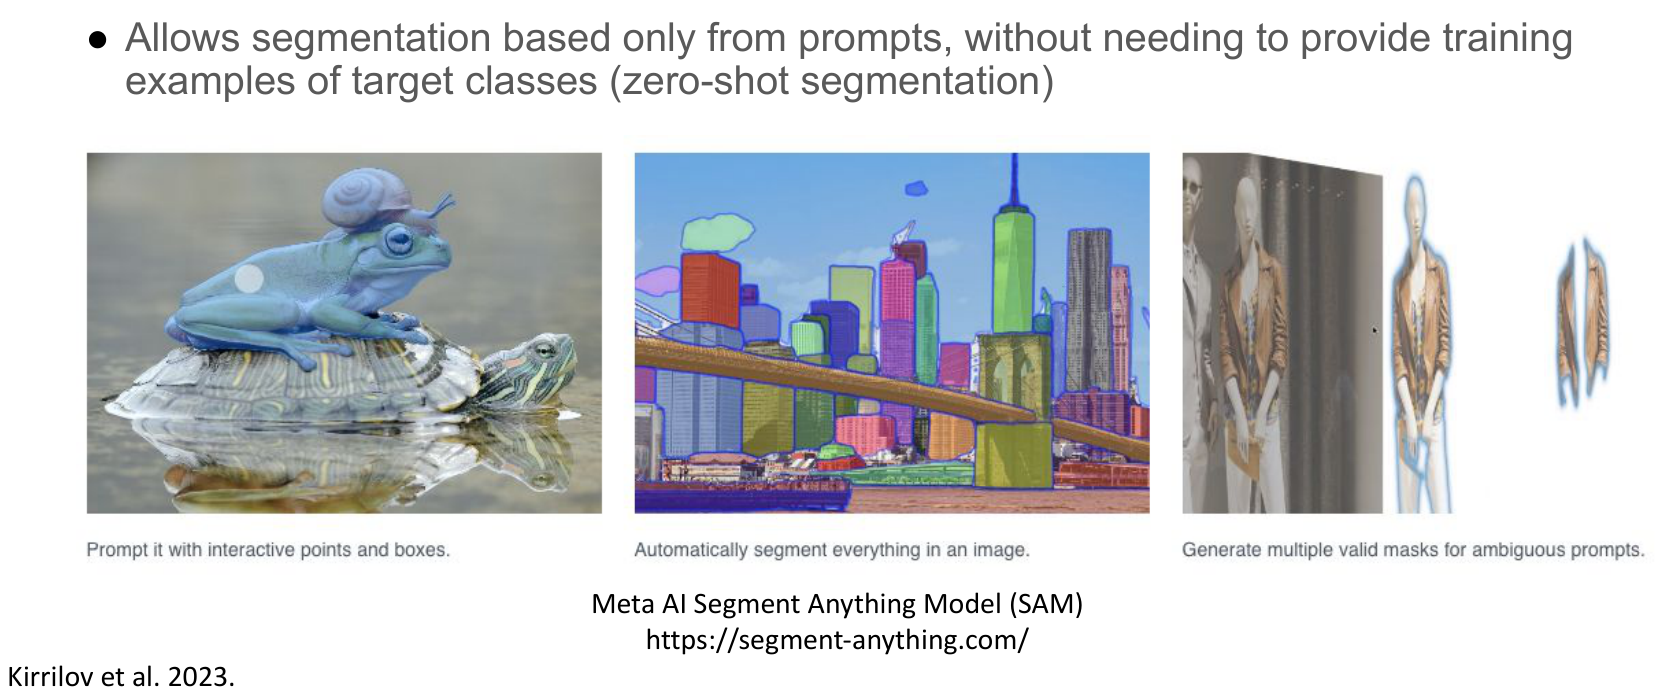
\includegraphics[width=\textwidth,height=0.80\textheight,keepaspectratio]{images/foundation-models/sam_zero_shot_segmentation_examples.png}\\[0.1em]
  {\scriptsize Stanford BIODS 276, Lecture 1 (S.\ Yeung-Levy); examples from \href{https://segment-anything.com/}{segment-anything.com}.}
\end{frame}



\begin{frame}{How Does SAM Work?}
  \begin{itemize}
    \item A heavy \textbf{image encoder} (MAE-pretrained ViT) embeds the image once; a light \textbf{prompt encoder} and \textbf{mask decoder} then run interactively in milliseconds.
    \item User or downstream model provides prompts (points, boxes, masks).
    \item The decoder predicts \textbf{several candidate masks} to resolve ambiguous prompts (a click on a shirt could mean the shirt or the person).
    \item Produces high-quality object masks across a wide range of settings without fine-tuning; masks are class-agnostic (no labels attached).
  \end{itemize}
  \centering
  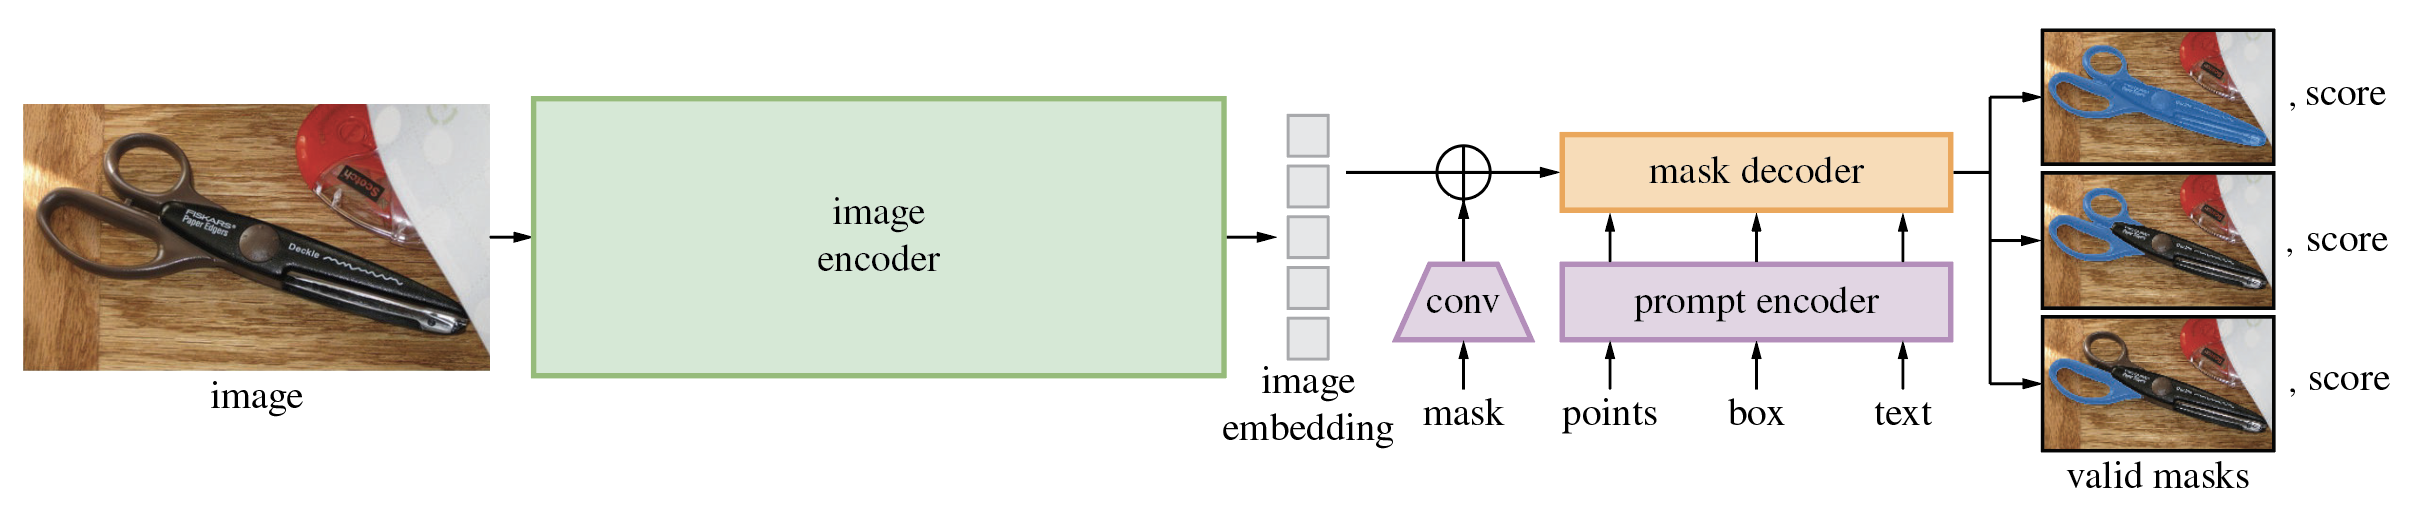
\includegraphics[width=0.85\textwidth]{images/foundation-models/sam_schema.png}\\[0.1em]
  {\scriptsize Kirillov et al., ``Segment Anything,'' ICCV 2023, Fig.~4.}
\end{frame}

% --- SAM 1: data engine and SA-1B ---
\begin{frame}{SAM 1: The Data Engine Behind SA-1B}
  \begin{itemize}\itemsep0.3em
    \item There was no billion-mask dataset to train on, so Meta built one \textbf{with the model in the loop}, in three stages:
    \begin{enumerate}\itemsep0.15em
      \item \textbf{Assisted-manual:} annotators refine masks proposed by an early SAM.
      \item \textbf{Semi-automatic:} SAM proposes confident masks; annotators add what it missed.
      \item \textbf{Fully automatic:} SAM is prompted with a grid of points and annotates images alone.
    \end{enumerate}
    \item Result: \textbf{SA-1B} with 11M licensed images and \textbf{1.1B masks}, orders of magnitude larger than prior segmentation datasets.
    \item The pattern (model annotates, humans verify, retrain, repeat) recurs in SAM 2 and SAM 3; for foundation models, the \textbf{data engine} is as important as the architecture.
  \end{itemize}
\end{frame}

% --- SAM 2: video and streaming memory ---
\begin{frame}{SAM 2: Promptable Segmentation in Video}
  \begin{itemize}\itemsep0.3em
    \item Extends promptable segmentation to \textbf{video}: prompt on any frame, and the model propagates the object mask (a \emph{masklet}) through the clip.
    \item \textbf{Streaming memory:} a memory bank stores features and object pointers from past frames; each new frame \textbf{cross-attends} to this memory before decoding its mask.
    \item Corrections are interactive: extra clicks on any frame refine the whole track.
    \item Trained with its own data engine, producing the \textbf{SA-V} dataset ($\sim$51K videos, $\sim$600K masklets); also faster than SAM 1 on still images.
  \end{itemize}
\end{frame}

\begin{frame}{SAM 1, SAM 2, and SAM 3: What's the Difference?}
  \begin{columns}[T,onlytextwidth]
    \begin{column}{0.32\textwidth}
      \textbf{SAM 1}
      \begin{itemize}\footnotesize
        \item Segments any object in any image.
        \item Requires as little as a single click to segment an object.
        \item Refine prediction with a few clicks.
      \end{itemize}
    \end{column}
    \begin{column}{0.32\textwidth}
      \textbf{SAM 2}
      \begin{itemize}\footnotesize
        \item Segments and tracks any object in any image or video.
        \item Uses click, box, or mask prompts.
        \item Tracks segment predictions across video frames.
        \item Refine prediction with a few clicks.
      \end{itemize}
    \end{column}
    \begin{column}{0.32\textwidth}
      \textbf{SAM 3}
      \begin{itemize}\footnotesize
        \item Detect, segment, and track every instance of any object category in an image or video.
        \item Uses text or examples as prompts.
        \item Segments and tracks objects from a click.
        \item Tracks segment predictions across frames.
        \item Detects and segments matching instances.
        \item Refine detection with visual examples.
      \end{itemize}
    \end{column}
  \end{columns}
\end{frame}


\begin{frame}{SAM 3 Architecture: Data Engine}
  \centering
  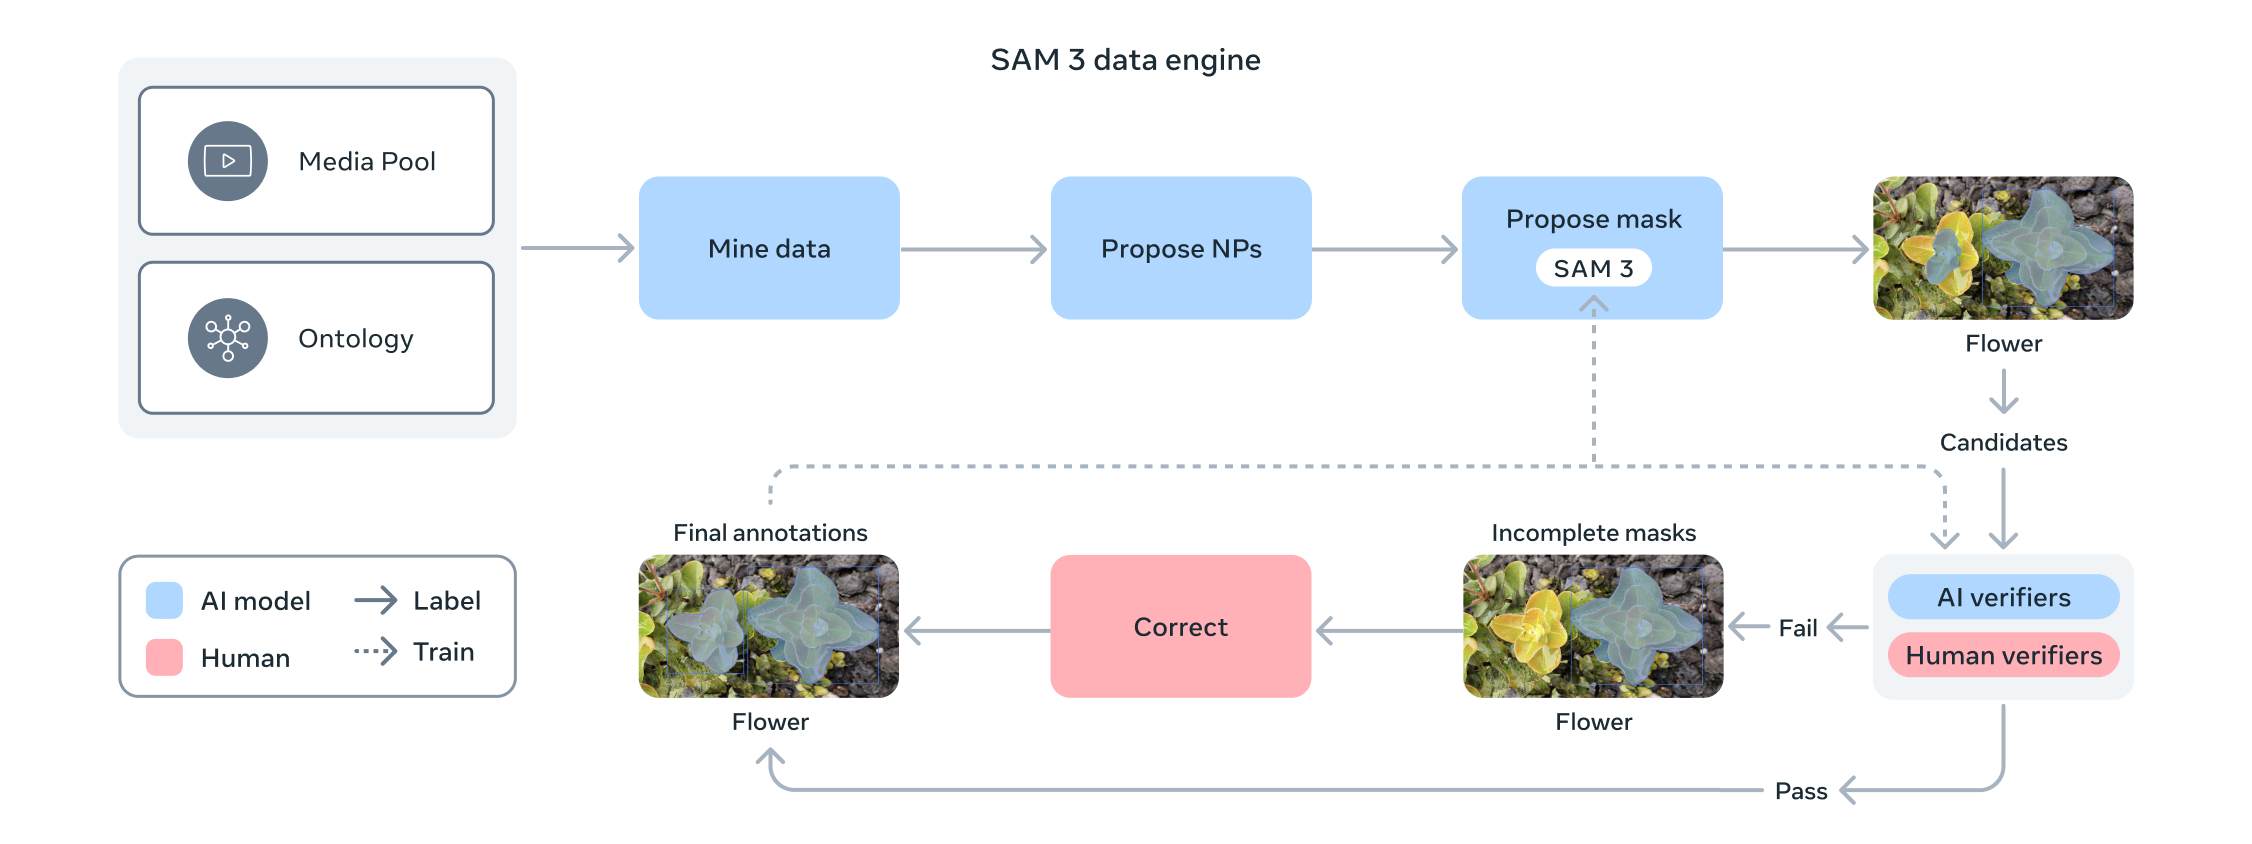
\includegraphics[width=0.82\textwidth, height=0.86\textheight, keepaspectratio]{images/foundation-models/sam3_data_engine.png}\\[0.1em]
  {\scriptsize SAM 3 data-engine loop from the Meta AI blog, ``SAM 3.1'' (\url{https://ai.meta.com/blog/segment-anything-model-3/}).}
  \vspace{0.2em}
  \begin{itemize}\footnotesize
    \item Getting masks \emph{with text labels} across many categories and domains is the hard part; SAM 3 scales the SAM data-engine pattern to concepts.
    \item AI models and annotators (human and Llama-based) collaborate in a feedback loop to mine, annotate, and verify data, yielding \textbf{4M+} annotated concepts across diverse domains.
  \end{itemize}
\end{frame}


\begin{frame}{SAM 3 Architecture: Core Model}
  \centering
  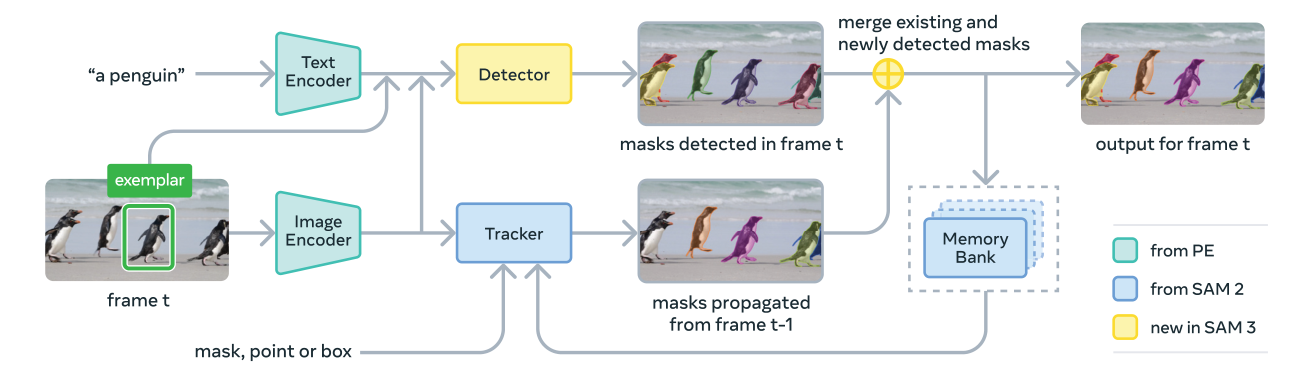
\includegraphics[width=0.82\textwidth, height=0.86\textheight, keepaspectratio]{images/foundation-models/sam3_page4_architecture_overview.png}\\[0.15em]
  {\scriptsize SAM 3 model summary and detector/tracker architecture. [Carion et al., ``SAM 3: Segment Anything with Concepts,'' 2025, Fig.~4]}\\[0.2em]
  \footnotesize
  A dual encoder-decoder transformer serves as the \textbf{detector} for image-level capabilities and is used together with a \textbf{tracker} and memory for video. Both receive vision-language features from an aligned Perception Encoder (PE) backbone.
\end{frame}


\begin{frame}{SAM 3.1 Inference Architecture: Object Multiplexing}
  \centering
  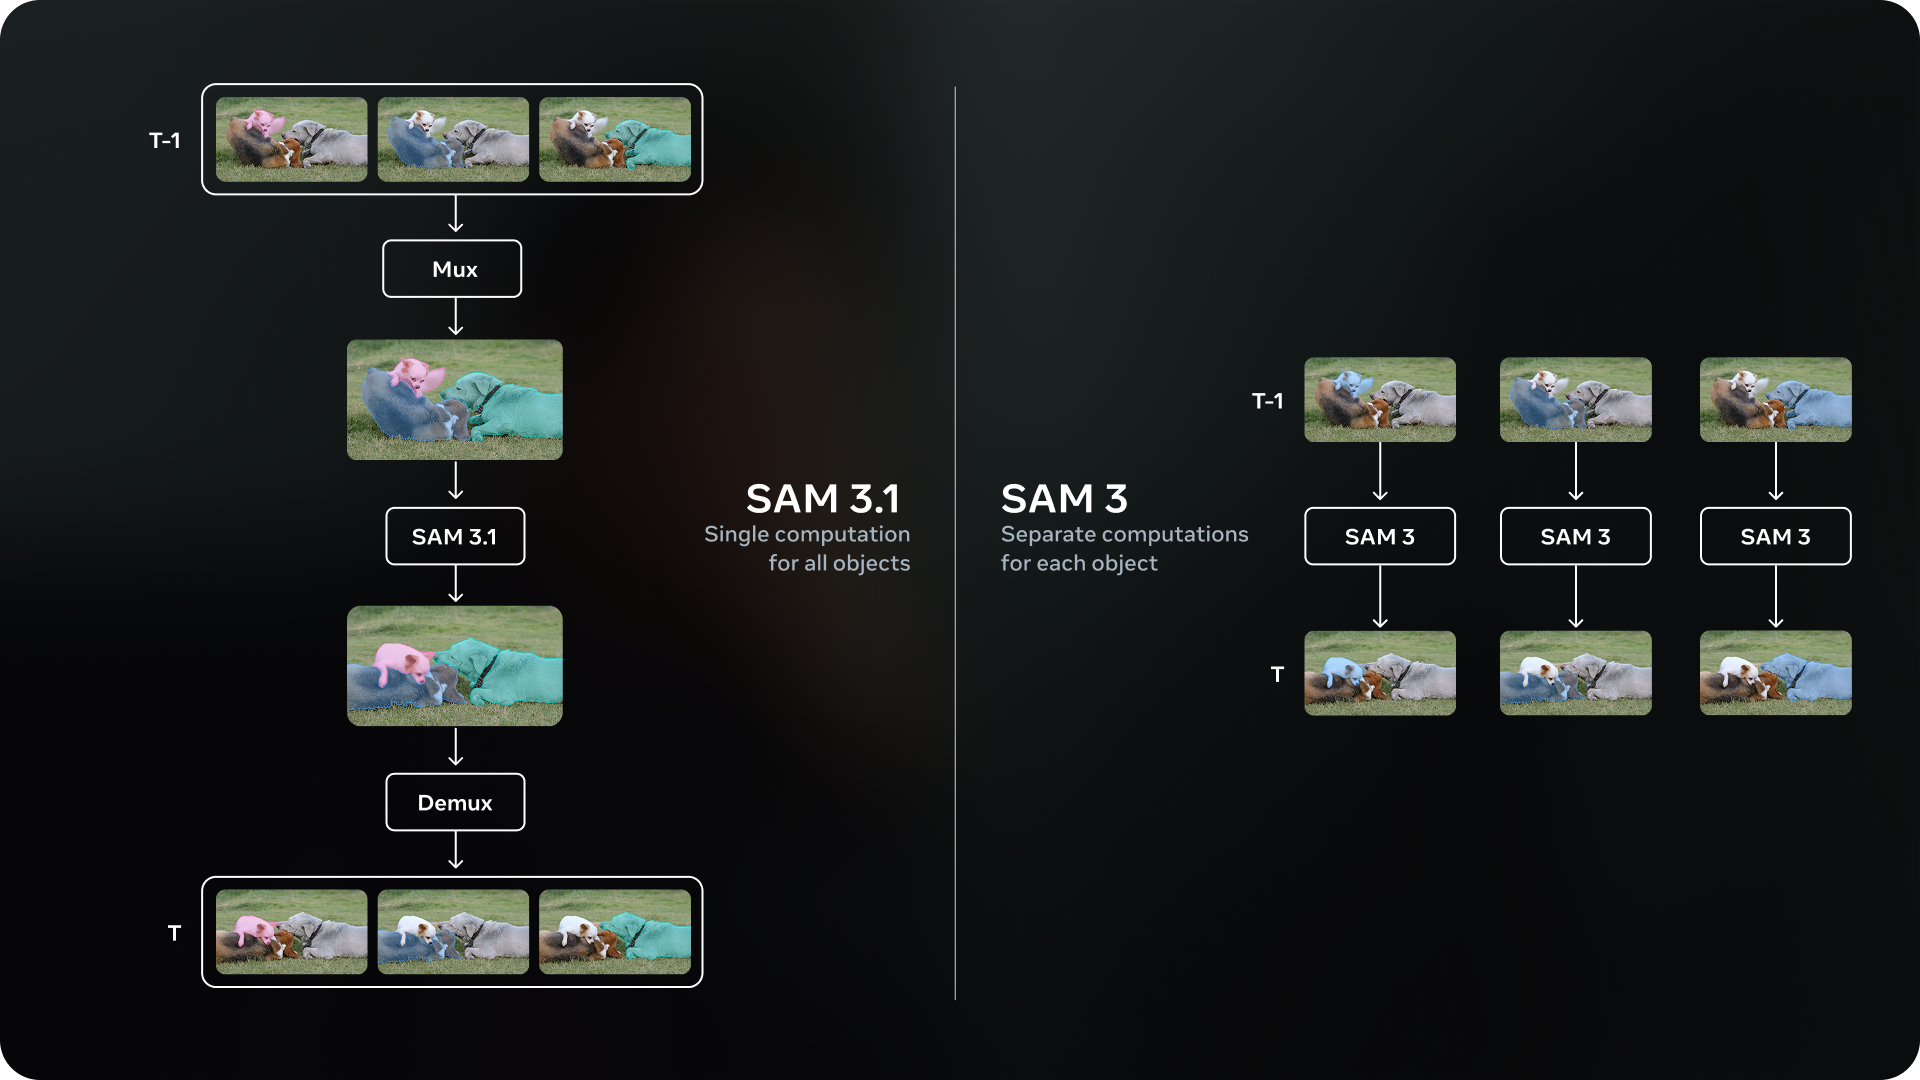
\includegraphics[width=0.68\textwidth, height=0.6\textheight, keepaspectratio]{images/foundation-models/sam3_vs_sam31_video_computation.png}\\[0.1em]
  {\scriptsize SAM 3.1 multiplexed inference versus per-object computation. [Source: Meta AI blog, ``SAM 3.1,'' \url{https://ai.meta.com/blog/segment-anything-model-3/}]}
  \vspace{0.2em}
  \begin{itemize}\footnotesize
    \item Process multiple tracked objects in one forward pass (\emph{multiplexing}) instead of one pass per object.
    \item Shared object-level context reduces redundant compute and helps crowded-scene tracking.
  \end{itemize}
\end{frame}
